\documentclass[12pt]{tcc} 

\usepackage[english]{babel} 
\usepackage[english]{babel}
\usepackage[T1]{fontenc}
\usepackage{datetime2}
\DTMsetdatestyle{ddmmyyyy}
\usepackage{algorithm}
\renewcommand{\algorithmcfname}{Algorithm}
\usepackage[noend]{algpseudocode}

\graphicspath{{./figures/}}

% Informações do trabalho
\newcommand\dtitle{{\normalsize\mdseries as part of Research Internship}}

\newcommand\dauthor{Maurya Samanta\\UG-4,\\Department of Production Engineering,\\Jadavpur University}


\newcommand\dadvisor{Dr. Rajib Das\\ Department of Computer Science and Engineering,\\ University of Calcutta}

% Definição de acronimos

\makeglossaries

\newacronym{TCC}{TCC}{Trabalho de Conclusão de Curso}
\addto\captionsenglish{\renewcommand{\chaptername}{}}

\begin{document}
	\pagenumbering{gobble}
	\pagenumbering{roman}
	
	\dcover
	
	\dtables
	
	
	
	
	\pagenumbering{arabic}
	\justifying
	
	\chapter{Introduction}
	\label{sec_introducao}
	
	
	
	Cloud computing refers to the delivery of computing services—including servers, storage, databases, networking, software, analytics, and intelligence—over the internet. Since the early 21st century, it has experienced rapid growth, becoming a foundational technology for supporting large-scale applications targeting global markets. Cloud platforms offer unparalleled scalability, flexibility, and cost-efficiency, making them ideal for organizations seeking to offload infrastructure management and focus on application-level concerns.
    
	In the Infrastructure-as-a-Service (IaaS) model, cloud providers offer a wide variety of virtual machines (VMs) with different performance capabilities and pricing structures. Users can rent these VMs on a pay-as-you-go basis, meaning they are charged only for the resources consumed during execution. This model is especially suitable for applications such as scientific workflows, where computational tasks can be mapped onto cloud resources without requiring upfront infrastructure investment.
    
	High-performance VMs, though more expensive, can execute tasks faster than their lower-performance counterparts. Therefore, users must often strike a trade-off between execution time and monetary cost. A common objective is to complete a given workflow within a user-defined deadline while minimizing the total cost incurred. This leads to a fundamental optimization problem in workflow scheduling, where the selection of VM types and task assignments must balance speed and cost.
    
	However, cloud resources are not perfectly reliable. Failures may occur due to hardware faults, network issues, or transient errors. As a result, users may not only care about cost and execution time but also about the probability of successful completion, i.e., the reliability of their workflows. 
    
	This introduces an additional dimension to the scheduling problem: ensuring cost-effective execution within the deadline, while maintaining a target reliability level. Designing algorithms that satisfy all three constraints—cost, deadline, and reliability—is a complex but essential challenge in cloud workflow management.

	
	\chapter{Problem Statement}
	\label{sec_fund_teorica}
	
	A scientific workflow consists of a set of tasks \( \{t_1, t_2, t_3, \ldots, t_n\} \), where dependencies exist between tasks. Specifically, a task \( t_x \) is said to depend on a task \( t_y \) if the input resources of \( t_x \) are a subset of the output resources of \( t_y \). Thus, the workflow can be mathematically modeled as a Directed Acyclic Graph (DAG). Let \( T \) be the set of all tasks, and let \( E \subseteq T \times T \) be the set of directed edges that represent the dependencies. Each edge \( e_{i,j} = (t_i, t_j) \in E \) represents a precedence constraint, indicating that task \( t_j \) can start execution only after task \( t_i \) has completed. For any task \( t_i \), the set of its immediate predecessors is denoted by \( \text{parent}(t_i) \), and the set of its immediate successors is denoted by \( \text{child}(t_i) \). A task with no parent, i.e., \( \text{parent}(t_i) = \varnothing \), is called an entry task. A task with no child, i.e., \( \text{child}(t_i) = \varnothing \), is called an exit task. Each task \( t_i \) is associated with a set of input files, denoted by \( \text{inputfiles}(t_i) \), a set of output files, \( \text{outputfiles}(t_i) \), and an expected runtime. The files shared between tasks are assumed to have defined storage sizes, typically measured in bytes.

	
A set of virtual machines \(VM = \{\text{VM}_1, \text{VM}_2, \text{VM}_3, \ldots, \text{VM}_n\} \) is provisioned to clients by Infrastructure-as-a-Service (IaaS) providers. Each virtual machine is characterized by a unique identifier, a fixed storage capacity (in gigabytes), a number of virtual CPUs (vCPUs), network bandwidth (in megabytes per second), and an associated on-demand cost (in USD per hour). The configuration of a VM directly influences its cost; that is, machines with higher computational capabilities incur higher charges. The computational power of a VM is typically expressed in terms of Million Instructions Per Second (MIPS). For a given virtual machine \( \text{VM}_i \), the MIPS value is calculated as shown in Equation~\eqref{eq:mips}:

\begin{equation}
\text{MIPS}(\text{VM}_i) = \text{vCPU}_i \times \text{ClockSpeed}_i \times 1000
\label{eq:mips}
\end{equation}

\noindent where \( \text{vCPU}_i \) is the number of virtual CPUs allocated to \( \text{VM}_i \), and \( \text{ClockSpeed}_i \) is the clock frequency (in GHz) of each vCPU.

	Each virtual machine \( \text{VM}_i \) is associated with a fault probability, denoted as \( F_i \), which quantifies the likelihood of failure during task execution. This probability is modeled as an exponential decay function with respect to execution time, given by Equation~\eqref{eq:fault-prob}:

\begin{equation}
F_i = e^{-\lambda t}
\label{eq:fault-prob}
\end{equation}

\noindent where \( \lambda \) is a constant representing the failure rate, and \( t \) is the runtime of a specific task on \( \text{VM}_i \).

To mitigate the risk of failure, tasks can be replicated across multiple virtual machines with similar performance characteristics. Let \( x_i \) denote the number of such replications. The net fault probability after replication becomes:

\begin{equation}
F_n_e_t=F_i^{x_i}
\label{eq:net-fault}
\end{equation}

\noindent Consequently, the success probability of the task (i.e., the probability that at least one replica completes successfully) is given by:

\begin{equation}
S_i=1 - F_i^{x_i}
\label{eq:success-prob}
\end{equation}

	It is assumed that the VMs are totally responsible for running the workflows as well storing the input/output files. It is assumed that any number of VM instances can be launched from VM set i.e. there is no restriction on the leasing of the number of VM instances. Also, Cloud computing follows the pay-per-use model which means users are being charged for whole time duration even if they use only a fraction it. Thus, in the proposed model, each instance of leased VM is charged per second time interval. Bandwidth costs are involved in transferring files from one VM to another.

    The objective of this work is to determine an optimal mapping of the task set \( T \) of a workflow onto a set of virtual machine instances derived from a given set of VM configurations (\( \text{VM}_{\text{set}} \)), such that both the total price for execution (TPE) and the total execution time (TET) are minimized. This must be achieved while adhering to the user-defined deadline, satisfying the precedence constraints among tasks, and ensuring the required reliability of the workflow.
\begin{equation}
\begin{aligned}
\text{Minimize:} \quad & \text{TPE} = \sum_i c_i t_i x_i \\
\text{Subject to:} \quad & \prod_i S_i \geq R_w \\
& \sum_i t_i \leq D
\end{aligned}
\label{eq:optimization}
\end{equation}

\noindent
where:
\begin{itemize}
    \item \( c_i \): Cost of executing the task on a VM of type \( i \),
    \item \( t_i \): Runtime of the task on VM type \( i \),
    \item \( x_i \): Number of replications of the task on VM type \( i \),
    \item \( S_i \): Success probability of the task after replication,
    \item \( R_w \): Required reliability of the entire workflow,
    \item \( D \): User-defined deadline.
\end{itemize}

	
	
	\chapter{Solution}
	\label{sec_solution}
	
	The proposed algorithm determines the most cost-effective schedule for executing a workflow within a user-defined deadline, while satisfying a specified reliability constraint. The solution employs Lagrange Multiplier Optimization to solve the constrained optimization problem described in Equation~\eqref{eq:optimization}. The algorithm consists of two main components: the \textbf{VM Allocation Algorithm} and the \textbf{Task Replication Algorithm}.

\subsection*{VM Allocation Algorithm}

Table~\ref{tab:notations} presents the key notations used in this work. Below are the definitions and mathematical formulations of important scheduling metrics:
\begin{itemize}

    \item \textbf{Earliest Start Time (\( \text{EST}_{k,i} \))}:
    The earliest time at which task \( t_i \) can begin execution on VM \( k \), given that all parent tasks have finished and data has been transferred.  
    \begin{equation}
    \text{EST}_{k,i} = \max_{t_j \in \text{parent}(t_i)} \left( \text{EFT}_{j} + \text{CD}_{j,i} \right)
    \end{equation}

    \item \textbf{Earliest Finish Time (\( \text{EFT}_{k,i} \))}:  
    The time at which task \( t_i \) will complete execution on VM \( k \), assuming it starts at \( \text{EST}_{k,i} \).  
    \begin{equation}
    \text{EFT}_{k,i} = \text{EST}_{k,i} + \frac{\text{MI}(t_i)}{\text{MIPS}(\text{VM}_k)}
    \end{equation}

    \item \textbf{Communication Delay (\( \text{CD}_{i,j} \))}:  
    The time required to transfer data between tasks \( t_i \) and \( t_j \) if scheduled on different VMs.  
    \begin{equation}
    \text{CD}_{i,j} =
    \begin{cases}
    \dfrac{\text{data\_size}_{i,j}}{\max(\text{bandwidth}(\text{VM}_i),\ \text{bandwidth}(\text{VM}_j))}, & \text{if } \text{VM}(t_i) \neq \text{VM}(t_j) \\
    0, & \text{otherwise}
    \end{cases}
    \end{equation}

    \item \textbf{Upward Rank (\( r_{u,i} \))}:  
    The length of the longest path from task \( t_i \) to an exit task in the workflow DAG, considering average computation and communication costs.  
    \begin{equation}
    r_{u,i} = \text{runtime}(t_i) + \max_{t_j \in \text{child}(t_i)} \left( \overline{CD}_{i,j} + r_{u,j} \right)
    \end{equation}

    \item \textbf{Sub-deadline (\( D_i \))}:  
    The sub-deadline of a task \( t_i \) is defined as:
    \begin{equation}
    D_i = \frac{r_{u,i}}{r_{u,\text{entry}}} \times D
    \end{equation}

    \item \textbf{Cost (\( C_{k,i} \))}:  
    The monetary cost of executing task \( t_i \) on virtual machine \( \text{VM}_k \).  
    \begin{equation}
    C_{k,i} = \frac{\text{MI}(t_i)}{\text{MIPS}(\text{VM}_k)} \times \left( \frac{\text{price}(\text{VM}_k)}{3600} \right)
    \end{equation}

\end{itemize}


\begin{table}[H]
\centering
\caption{Notations Used in the VM Allocation Algorithm}
\label{tab:notations}
\begin{tabular}{|c|l|}
\hline
\textbf{Symbol} & \textbf{Description} \\
\hline
\( D \) & User-defined deadline in miliseconds \\
\( \text{EST}_{k,i} \) & Earliest start time of \( t_i \) on VM \( k \) \\
\( \text{EFT}_{k,i} \) & Earliest finish time of \( t_i \) on VM \( k \) \\
\( \text{CD}_{i,j} \) & Communication delay between \( t_i \) and \( t_j \) \\
\( MI_{i} \) & Million Instructions of task \( t_i \) \\
\( MIPS_{k} \) & Million Instructions Per Second of VM \( VM_k \) \\
\( datasize_{i,j} \) & Total data to be transferred from task \( t_i \) to task \( t_j \) in MB \\
\( child(t_i) \) & Set of all dependance tasks(children) of task \( t_i \) \\
\( r_{u,i} \) & Upward Rank of task \( t_i \) \\
\( C_{k,i} \) & Cost of executing \( t_i \) on VM \( k \) in USD \\
\( price(VM_k) \) & On-demand pricing of VM \(VM_k\) in USD/hour \\
\hline
\end{tabular}
\end{table}
Algorithm~\ref{alg:highlevel} describes the high-level flow of the scheduler algorithm. After some initialization, the upward ranks of the tasks are calculated using Equation~(3.4). Subsequently, sub-deadlines for each task are estimated using Equation~(3.5). For each task, a set of eligible VMs is prepared. The eligibility of VMs is determined based on two criteria: the total storage required by the task (sum of input and output file sizes), and the runtime of the task on the VM compared to its assigned sub-deadline. Algorithm~\ref{alg:eligibleVMs} presents the logic used for estimating eligible virtual machines for a task.

By estimating eligible virtual machines (VMs) in advance, the scheduling process is significantly optimized. Instead of evaluating every task on all available VMs, the algorithm restricts scheduling decisions to only those VMs that meet the task’s resource requirements. This pre-filtering step not only reduces computational overhead but also contributes to cost efficiency, as it ensures that only feasible and capacity-sufficient VMs are considered during allocation.


\begin{algorithm}[H]
\caption{Workflow Scheduling Main Procedure}
\begin{algorithmic}[1]
\Require DAG workflow in XML format containing $n$ tasks 
\Require VM dataset with $k$ virtual machines
\Ensure A cost-optimized, deadline-aware task schedule with reliability

\State taskMap $\gets$ \texttt{parseXML()}
\State topoSortedJobs $\gets$ \texttt{topologicalSort(taskMap)}
\State upwardRanks $\gets$ \texttt{calculateUpwardRanks(topoSortedJobs)} according to Equation (3.4)
\State assignSubdeadlines(upwardRanks) according to Equation (3.5)
\State getEligibleVMs(topoSortedJobs, vms)
\State totalCost $\gets$ \texttt{schedule(topoSortedJobs)}
\State \texttt{Display}(totalCost)
\end{algorithmic}
\label{alg:highlevel}
\end{algorithm}

\begin{algorithm}[H]
\caption{Eligible VM Estimation}
\label{alg:eligibleVMs}
\begin{algorithmic}[1]
\Require List of tasks sorted according to upward ranks
\Require List of available VMs
\Ensure Estimate eligible VMs for each task

\For{each task \( j \) in tasks}
    \State Initialize \( \text{eligibleVMs}_j \gets [\ ] \)
    \State Compute \( \text{requiredStorage} \) from input/output files
    \For{each VM \( v \) in VMs}
        \State Compute \( \text{runtime} \gets \frac{\text{MI}(j)}{\text{MIPS}(v)} \)
        \If{\( \text{runtime} < \text{subDeadline}(j) \) \textbf{and} requiredStorage fits in \( v \)}
            \State Add \( v \) to \( \text{eligibleVMs}_j \)
        \EndIf
    \EndFor
    \State Assign \( \text{eligibleVMs}_j \) to job \( j \)
\EndFor
\end{algorithmic}
\end{algorithm}

Algorithm~\ref{alg:scheduler} outlines the core scheduling logic. For each virtual machine (VM), a tracking map is maintained to record the tasks assigned to it along with their respective start and finish times. This information is later used to compute the total cost of utilizing that VM.

For every task in the \texttt{UpwardRankSortedJobs} list, initial values for minimum cost, earliest start time (EST), and earliest finish time (EFT) are set to zero. The algorithm then iterates over the pre-estimated eligible VMs for the current task. Each task is tentatively scheduled on all its eligible VMs to evaluate the associated execution cost. The VM offering the lowest cost is selected for the task, and the VM-task schedule map is updated accordingly. During scheduling, the bandwidth cost is taken care of when the parent of the present task has been executed on a different Virtual Machine.

	\begin{algorithm}[H]
\caption{Task Scheduling with Cost Minimization}
\label{alg:scheduler}
\begin{algorithmic}[1]
\Require Sorted task list by upward rank \( \mathcal{J} \), list of VMs \( \mathcal{V} \),  VM availability map, file size and dependency maps

\State Initialize totalCost \( \gets 0 \)
\State Initialize schedule list \( \mathcal{S} \gets [\ ] \)

\State Initialize vmTaskMap for each \( \text{VM} \in \mathcal{A} \) with empty list

\For{each task \( t \in \mathcal{J} \)}
    \State \( \text{minCost} \gets \infty \), \( \text{bestVM} \gets \text{null} \)
    \State \( \text{bestEST} \gets 0 \), \( \text{bestEFT} \gets 0 \)

    \For{each VM \( v \in \text{eligibleVMs}(t) \)}
        \State \( \text{est} \gets \text{vmAvailability}[v] \)
        \For{each parent task \( p \in \text{parents}(t) \)}
            \If{\( p \) is scheduled}
                \State \( \text{commTime} \gets 0 \)
                \If{\( \text{assignedVM}(p) \neq v \)}
                    \State Compute data size from file map
                    \State Compute bandwidth of \( v \)
                    \State \( \text{commTime} \gets \text{dataSize} / \text{bandwidth} \) using Equation (3.3)
                \EndIf
                \State \( \text{est} \gets \max(\text{est}, \text{endTime}(p) + \text{commTime}) \)  using Equation (3.1)
                
            \EndIf
        \EndFor

        \)
        \State Compute runtime \( \gets \text{MI}(t) / \text{MIPS}(v) \)
        \State Compute EFT \( \gets \text{est} + \text{runtime} \) using Equation (3.2)

        \If{\( \text{EFT} \leq \text{subDeadline}(t) \)}
            \State Compute billing-based cost of execution on VM \( v \)
            \State Compute normalized delay bias

            \If{cost is minimal or delay bias is better}
                \State Update \( \text{minCost}, \text{bestVM}, \text{bestEST}, \text{bestEFT} \)
            \EndIf
        \EndIf
    \EndFor

    \State Assign \( t \) to \( \text{bestVM} \), update scheduling records and costs
\EndFor

\State \Return Final schedule and total cost

\end{algorithmic}
\end{algorithm}

\subsection*{Task Replication Algorithm}
 \subsection*{Nature of the Optimization Problem}

The objective function 
\[
\sum_{i} c_i t_i x_i
\]
is linear in the decision variables \( x_i \). However, the reliability constraint
\[
\prod_{i} S_i = \prod_{i} (1 - f_i^{x_i}) \geq R_w
\]
is non-linear and multiplicative, since each success probability depends exponentially on \( x_i \). This product of non-linear functions introduces non-linearity into the constraint space.

Therefore, the optimization problem becomes non-linear due to the following reasons:
\begin{itemize}
    \item The presence of exponential terms \( f_i^{x_i} \) in the success probability expressions.
    \item The multiplicative form of the reliability constraint \( \prod_i (1 - f_i^{x_i}) \), which prevents direct linear optimization.
    \item The use of logarithmic transformations required to linearize or approximate the constraint.
\end{itemize}

\subsection*{Use of Lagrangian Optimization}

Lagrangian optimization is a powerful method to solve constrained optimization problems, particularly when:
\begin{itemize}
    \item The objective function and/or constraints are non-linear.
    \item Direct analytical or linear programming solutions are not feasible due to coupling between decision variables.
\end{itemize}
	
\subsection*{Lagrangian Formulation for Replica Count Optimization}

We aim to minimize the total price of execution (TPE) given by:
\[
\text{TPE} = \sum_{i} c_i t_i x_i
\]
subject to the reliability constraint:
\[
\prod_{i} (1 - f_i^{x_i}) \geq R_w
\]

This is a non-linear optimization problem due to the multiplicative nature of the reliability constraint. To make it tractable, we introduce a change of variables:
\[
y_i = f_i^{x_i} \quad \Rightarrow \quad x_i = \frac{\ln y_i}{\ln f_i}
\]

This transforms the reliability constraint into:
\[
\prod_i (1 - y_i) \geq R_w \quad \Rightarrow \quad \sum_i \ln(1 - y_i) \geq \ln R_w
\]

Assuming small values of \( y_i \), we approximate using the first-order Taylor expansion:
\[
\ln(1 - y_i) \approx -y_i \quad \Rightarrow \quad \sum_i y_i \leq \ln\left(\frac{1}{R_w}\right)
\]

Now, substitute the transformed variable into the cost function:
\[
\text{TPE} = \sum_i c_i t_i x_i = \sum_i A_i \ln y_i \quad \text{where} \quad A_i = \frac{c_i t_i}{\ln f_i}
\]

To solve the constrained minimization, we use the method of Lagrange multipliers. The Lagrangian is:
\[
\mathcal{L}(y_1, y_2, \dots, y_n, \lambda) = \sum_i A_i \ln y_i + \lambda \left( \sum_i y_i - \ln\left(\frac{1}{R_w}\right) \right)
\]

We now compute the partial derivatives with respect to each \( y_i \):
\[
\frac{\partial \mathcal{L}}{\partial y_i} = \frac{A_i}{y_i} + \lambda
\]

Setting the derivative to zero for optimality:
\[
\frac{A_i}{y_i} + \lambda = 0 \quad \Rightarrow \quad y_i = -\frac{A_i}{\lambda}
\]

This gives the expression of \( y_i \) in terms of the Lagrange multiplier \( \lambda \). The corresponding values of \( x_i \) are then computed in code using this gradient-based logic.

Algorithm~\ref{alg:optimize_replica_counts} presents the optimization of replica counts \( x_i \) for each task in a workflow, aiming to minimize the Total Price of Execution (TPE) under a global reliability constraint. It begins with a reliability-based estimation of the minimum number of replicas using exponential failure modeling for each task. Subsequently, it applies gradient-based updates combined with a penalty method to iteratively refine the replica counts. At each step, the gradients of cost and reliability are evaluated and balanced to ensure cost efficiency while satisfying the reliability constraint. This process continues until the overall system reliability requirement is fulfilled.


	\begin{algorithm}[H]
\caption{OptimizeReplicaCounts: Replica Optimization under Reliability Constraint}
\label{alg:optimize_replica_counts}
\begin{algorithmic}[1]
\Require List of Jobs \texttt{jobs}, List of VMs \texttt{vms}, Failure rate \texttt{lambda}, Deadline \texttt{deadline}, Required system reliability \texttt{requiredReliability}
\Ensure Replica counts \( x[i] \) for each job \( i \)

\State Initialize array \( x[i] \gets 1.0 \) for all jobs
\For{each job \( i \) in \texttt{jobs}}
    \If{no eligible VMs for job \( i \)}
        \State Set \( x[i] \gets 1.0 \) and continue
    \EndIf
    \State Determine fastest MIPS and cheapest cost from eligible VMs
    \State Compute runtime \( t_i \gets \frac{\texttt{job.mi}}{\texttt{fastestMIPS}} \)
    \State Compute task reliability \( r_i \gets e^{-\lambda \cdot t_i} \)
    \State Set target reliability per task \( r_{\text{target}} \gets \texttt{requiredReliability}^{1/n} \)
    \If{\( r_i \geq r_{\text{target}} \)}
        \State \( x[i] \gets 1.0 \)
    \Else
        \State Estimate minimum replicas:
        \[
        x[i] \gets \left\lceil \frac{\ln(1 - r_{\text{target}})}{\ln(1 - r_i)} \right\rceil
        \]
    \EndIf
\EndFor

\State Evaluate initial system reliability
\If{initial reliability \( \geq \texttt{requiredReliability} \)}
    \State \Return \( x \)
\EndIf

\State Initialize: \texttt{mu} (penalty multiplier), \texttt{learningRate}, \texttt{muLearningRate}, \texttt{maxIters}
\State Precompute fastestMIPS and cheapestCosts per job from eligible VMs

\For{iteration = 1 to \texttt{maxIters}}
    \State Compute current total cost and system reliability
    \State Calculate constraint violation: \( \texttt{requiredReliability} - \texttt{systemReliability} \)
    \If{violation \( > \varepsilon \)}
        \For{each job \( i \)}
            \State Compute runtime and failure rate \( f_i \)
            \State Compute cost gradient: \( \texttt{cheapestCosts}[i] \cdot \texttt{runtime} \)
            \State Compute reliability gradient:
            \[
            \frac{\partial R_{\text{sys}}}{\partial x[i]} \approx R_{\text{sys}} \cdot f_i^{x[i]} \cdot \ln(f_i) / (1 - f_i^{x[i]})
            \]
            \State Combine gradients to compute total gradient:
            \[
            \texttt{totalGradient} \gets \texttt{costGradient} - \texttt{penalty} \cdot \texttt{reliabilityGradient}
            \]
            \State Update:
            \[
            x[i] \gets \max\left(1.0, \min\left(10.0, x[i] - \texttt{learningRate} \cdot \texttt{totalGradient} \right)\right)
            \]
        \EndFor
        \State Update penalty multiplier: \( \texttt{mu} \gets \texttt{mu} + \texttt{muLearningRate} \cdot \texttt{violation} \)
    \Else
        \State Break (constraints satisfied)
    \EndIf
\EndFor

\State \Return final array \( x \)
\end{algorithmic}
\end{algorithm}

By employing this algorithm, the number of replicas required for each task is determined in advance. This proactive approach significantly reduces the overall execution cost, as it avoids the need to perform trial-and-error replication during the actual scheduling phase. Consequently, the optimal number of replicas can be estimated without executing tasks, leading to more efficient scheduling decisions.

The calculated replica counts are leveraged within the scheduler function to replicate tasks onto additional VMs selected from each task's \texttt{eligibleVMs} list, as outlined in Algorithm~\ref{alg:scheduler_with_replica_counts}. Replica assignment follows a similar strategy as primary task allocation—considering VM availability and data transfer delays to maintain execution feasibility. It is assumed that replicas are launched in parallel, provided that the selected VMs are available at the moment of scheduling. This parallelism ensures that the makespan of the overall workflow is minimally impacted, while enhancing reliability through redundancy.

To simulate the probabilistic nature of task execution on cloud VMs, a random number uniformly distributed in the range [0, 1] is generated for each task execution attempt. This value is compared against the computed reliability of the task on the selected VM. If the reliability is less than or equal to the generated random number, the task is considered to have successfully executed on that VM. Upon the first successful execution, no further replicas are scheduled or executed for that task, as a single successful instance suffices to generate the required output for its dependent tasks.

Conversely, if the execution fails (i.e., the random number is less than the task reliability), subsequent replicas are launched according to the precomputed replica count. If none of the replicas succeed in the current scheduling round, the replication loop is re-entered until at least one successful execution is achieved, thereby ensuring task-level fault tolerance and reliability compliance.


\begin{algorithm}[H]
\caption{Replica Assignment for Scheduled Tasks}
\label{alg:scheduler_with_replica_counts}
\begin{algorithmic}[1]
\Require Replica counts array \texttt{replicaCounts}, Eligible VMs for each task, Pre-scheduled task with assigned best VM
\Ensure Replicas are assigned to additional VMs, respecting deadlines and minimizing cost 

\State Let \( R_i \gets \texttt{replicaCounts}[i] \)
\If{ \( R_i < 1 \) } 
    \State \( R_i \gets 1 \)
\EndIf

\State Assign main task to \( \texttt{bestVM} \)
\State Update \( \texttt{startTime} \), \( \texttt{endTime} \), and availability of \( \texttt{bestVM} \)
\State Add main task to \( \texttt{schedule} \)

\State \( \texttt{replicasAdded} \gets 1 \)
\State Create list \( \texttt{candidateReplicas} \gets \texttt{eligibleVMs} \setminus \{ \texttt{bestVM} \} \)
\State Sort \( \texttt{candidateReplicas} \) by ascending \( \frac{\texttt{cost}}{\texttt{reliability}} \)

\State Initialize RNG with fixed seed
\State \( \texttt{successAchieved} \gets \texttt{false} \)

\For{ each \( \texttt{vm} \) in \( \texttt{candidateReplicas} \) }
    \If{ \( \texttt{replicasAdded} \geq R_i \ \textbf{or} \ \texttt{successAchieved} \) }
        \State \textbf{break}
    \EndIf

    \State Estimate \( \texttt{est} \gets \texttt{availability}[vm] \)
    \State Compute \( \texttt{runtime} \gets \frac{MI_i}{MIPS_{vm}} \)
    \State Compute \( \texttt{eft} \gets \texttt{est} + \texttt{runtime} \)

    \If{ \( \texttt{eft} > \texttt{subDeadline}_i \) }
        \State \textbf{continue}
    \EndIf

    \State Create a replica copy of task \( T_i \)
    \State Assign replica to \( vm \)
    \State Set replica's \( \texttt{startTime} \) and \( \texttt{endTime} \)
    \State Update \( \texttt{availability}[vm] \gets \texttt{eft} \)
    \State Add replica to schedule and VM-task map
    \State \( \texttt{replicasAdded} \gets \texttt{replicasAdded} + 1 \)

    \State Generate \( r \sim \mathcal{U}(0, 1) \)
    \State Compute reliability \( \rho \gets \exp(-\lambda \cdot \texttt{runtime}) \)
    \If{ \( \rho \leq r \) }
        \State \( \texttt{successAchieved} \gets \texttt{true} \)
    \EndIf
\EndFor

\end{algorithmic}
\end{algorithm}

	
	\chapter{Results} 
	\label{sec_result}

The proposed scheduling and replica optimization algorithm was evaluated using three scientific workflows: \textit{Montage}, \textit{Sipht}, and \textit{Epigenomics}. The virtual machine configurations were sourced from AWS EC2 instance data, ensuring realistic modeling of cost, performance, and network heterogeneity.

The VM dataset includes a range of instance types with varying compute power (measured in MIPS), bandwidth, and storage capacity. The median characteristics of the VM pool used in our simulations are as follows:
\begin{itemize}
    \item \textbf{Median MIPS}: 131871
    \item \textbf{Median Bandwidth}: 52 MBps
    \item \textbf{Median Storage}: 3333 GB
\end{itemize}

The performance of the proposed approach was analyzed under varying system reliability thresholds and deadline constraints. Key metrics observed include the Total Price of Execution (TPE) and end-to-end workflow reliability. 

Simulations were conducted on a local machine configured as follows:

\begin{itemize}
    \item \textbf{Operating System}: Windows 10
    \item \textbf{Processor}: 13th Gen Intel(R) Core(TM) i5-1335U (1.30 GHz)
    \item \textbf{Installed RAM}: 8.00 GB
    \item \textbf{System Type}: 64-bit operating system, x64-based processor
\end{itemize}

The workflows used in this simulation—\textit{Epigenomics}, \textit{Sipht}, and \textit{Montage}—each consist of 100 tasks. To evaluate the performance of the scheduling and replication strategy under varying temporal constraints, each workflow was executed across a range of 10 distinct deadlines. These deadlines were systematically derived by incrementally increasing the smallest time possible to execute the workflow by 10\% at each step.

\begin{itemize}
    \item \textbf{Epigenomics}: This workflow simulates a bioinformatics pipeline used for mapping and analyzing epigenetic markers such as DNA methylation. It involves several data preprocessing and alignment steps, characterized by moderate computation and communication requirements with parallel branches.

    \item \textbf{Sipht}: The Sipht workflow identifies and annotates non-coding RNAs in bacterial genomes. It consists of a large number of small, mostly independent tasks, making it suitable for evaluating task-level parallelism and replica assignment strategies.

    \item \textbf{Montage}: Montage is an astronomy workflow that generates custom science-grade astronomical image mosaics. It is highly I/O-intensive and exhibits a deep dependency structure, useful for evaluating scheduling efficiency under tight deadlines and data transfer constraints.
\end{itemize}

\begin{figure}[h!]
    \centering
    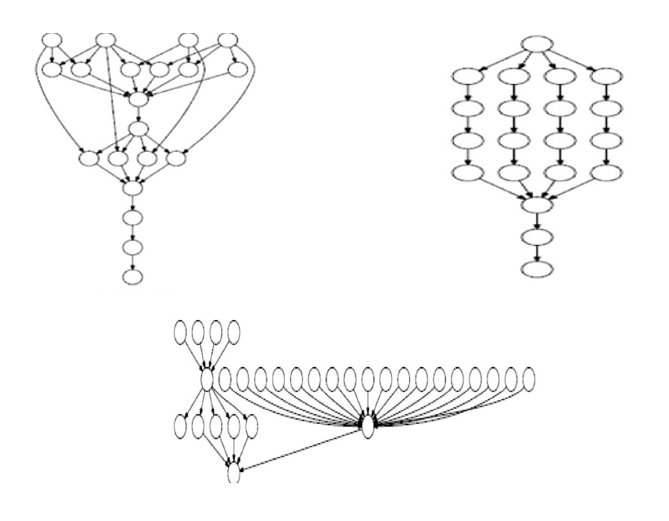
\includegraphics[width=0.8\textwidth]{figures/workflows.png}
    \caption{Workflow structures of Montage, Epigenomics and Sipht}
    \label{fig:workflow_structs}
\end{figure}

Given that the proposed algorithm computes task-level sub-deadlines based on Equation~(3.5), it follows that more relaxed (softer) workflow deadlines allow for proportionally larger sub-deadlines for individual tasks. This increased temporal flexibility enables the scheduler to assign tasks to a broader range of virtual machines, including cost-efficient but slower instances.

As a result, the observed trend in the cost-versus-deadline plots reflects a consistent decrease in total execution cost with softer deadlines. This behavior validates the effectiveness of the algorithm in exploiting temporal slack to reduce expenditure while maintaining system reliability.


\begin{figure}[h!]
    \centering
    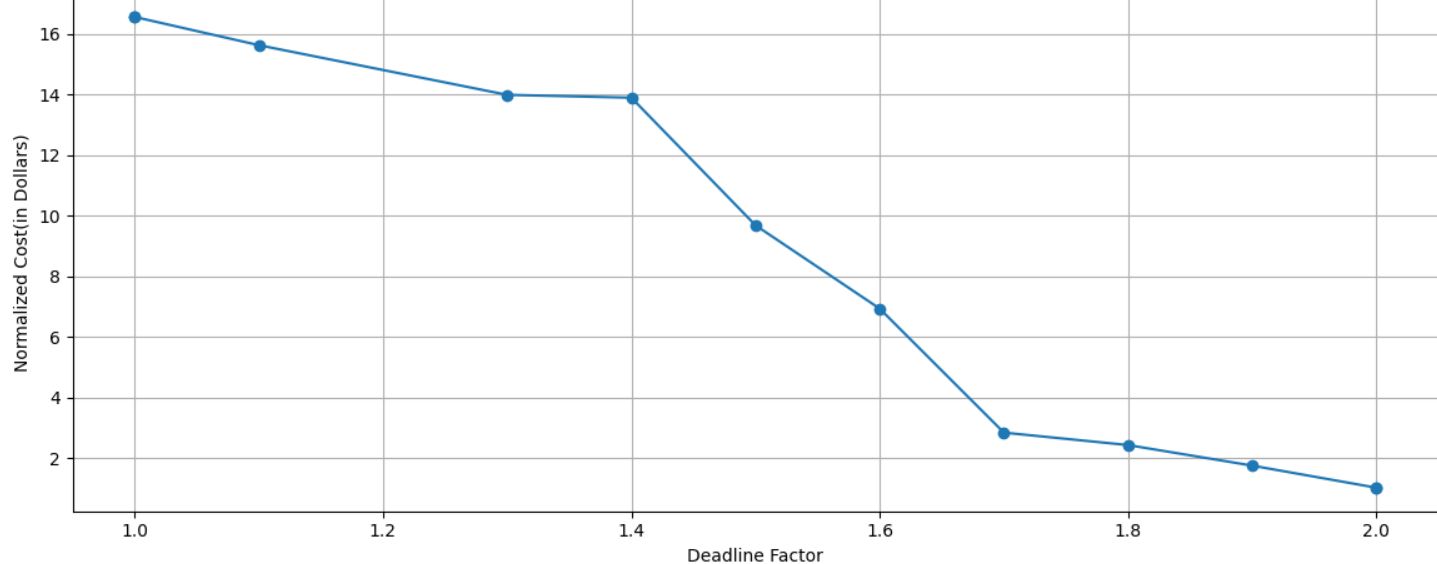
\includegraphics[width=0.8\textwidth]{figures/Montage.png}
    \caption{Effect of varying deadlines on total execution cost for the Montage workflow}
    \label{fig:montage-cost-deadline}
\end{figure}

\begin{figure}[h!]
    \centering
    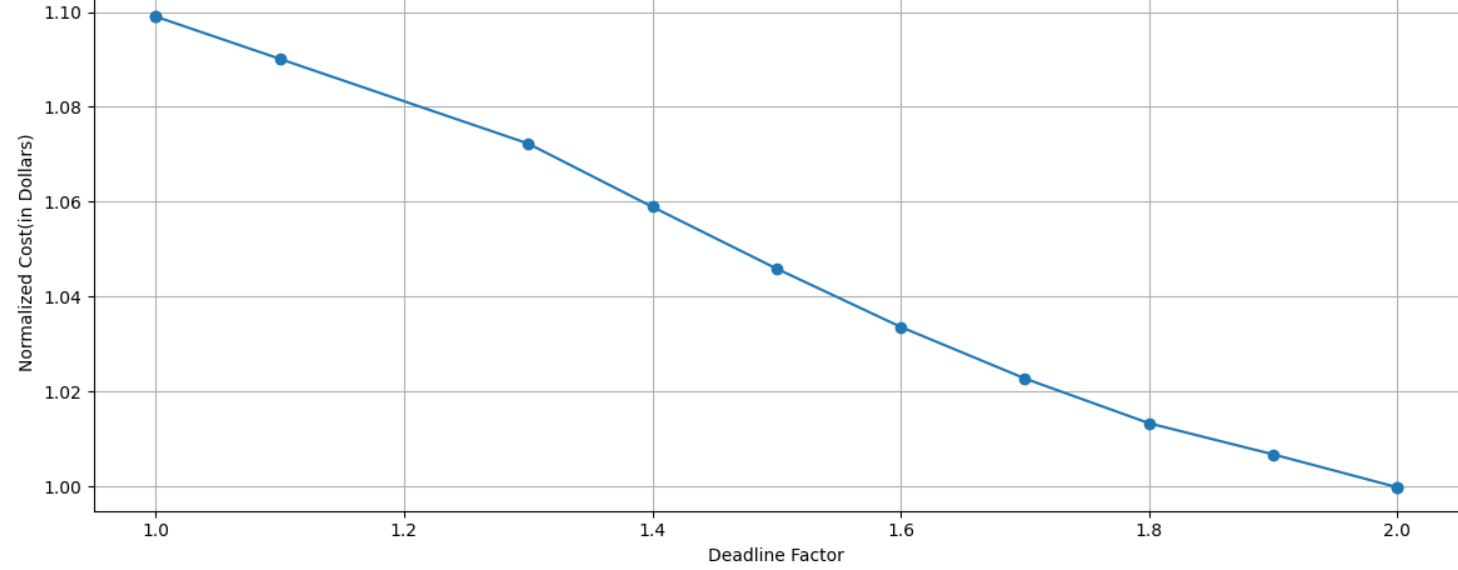
\includegraphics[width=0.8\textwidth]{figures/Epigenomics.png}
    \caption{Effect of varying deadlines on total execution cost for the Epigenomics workflow}
    \label{fig:epigenomics-cost-deadline}
\end{figure}

\begin{figure}[h!]
    \centering
    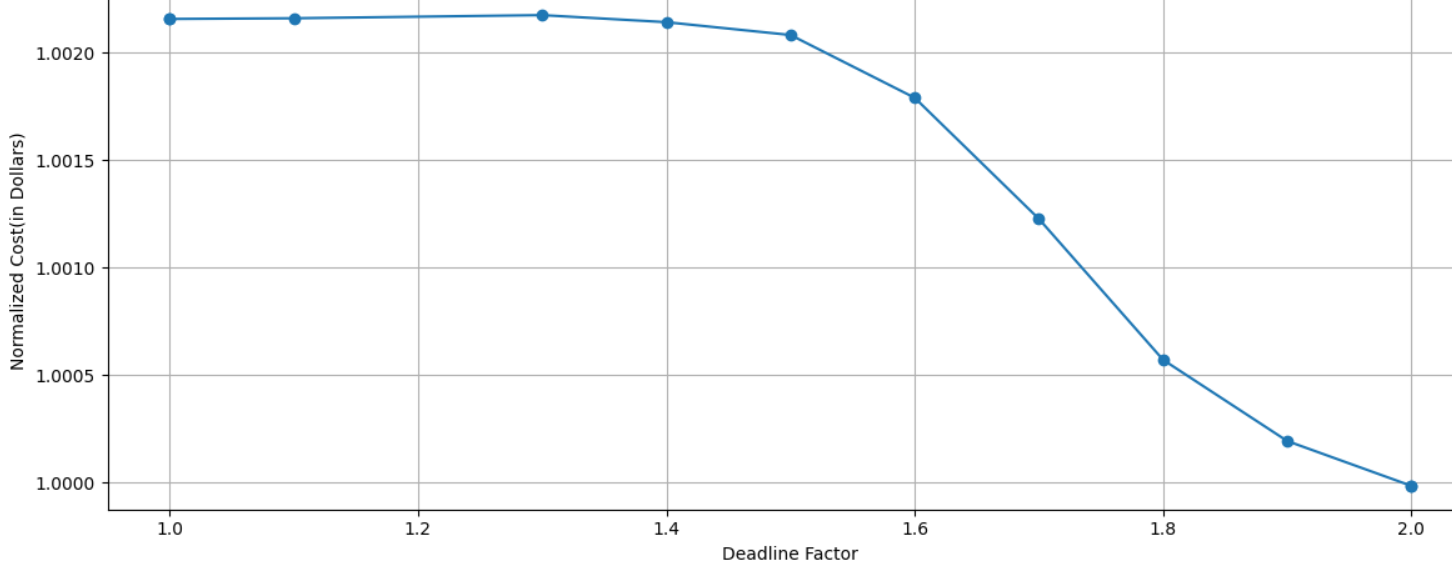
\includegraphics[width=0.8\textwidth]{figures/Sipht.png}
    \caption{Effect of varying deadlines on total execution cost for the Sipht workflow}
    \label{fig:sipht-cost-deadline}
\end{figure}
	
To evaluate the impact of reliability constraints on execution cost, the three workflows were simulated at reliability levels of 0.90, 0.95, and 0.99. For each reliability level, the workflows were executed across ten deadline settings, each incrementally relaxed by 10\% over the minimum possible makespan for the workflow. The average cost across these executions was recorded and plotted. 

A comparative analysis was conducted between the proposed Lagrangian-based replica optimization algorithm and a baseline iterative method. In the baseline approach, replication counts are determined dynamically during scheduling, leading to increased computational overhead and higher execution costs. In contrast, the proposed method estimates replica counts prior to scheduling, allowing for more efficient resource allocation and cost reduction.

\begin{figure}[h!]
    \centering
    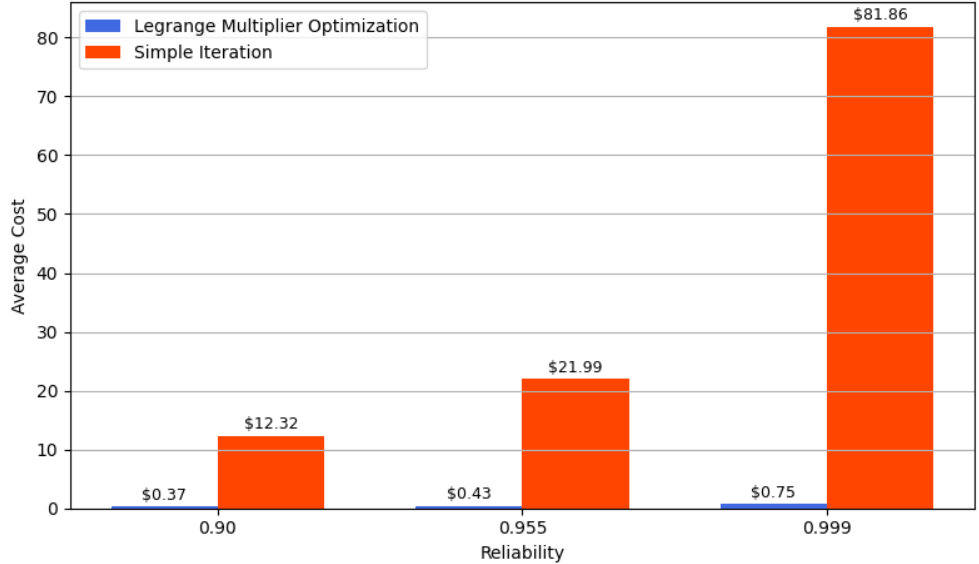
\includegraphics[width=0.8\textwidth]{figures/Mon_rel.png}
    \caption{Effect of varying reliability on total execution cost for the Montage workflow using proposed algorithm and iterative approach}
    \label{fig:montage-cost-rel}
\end{figure}

\begin{figure}[h!]
    \centering
    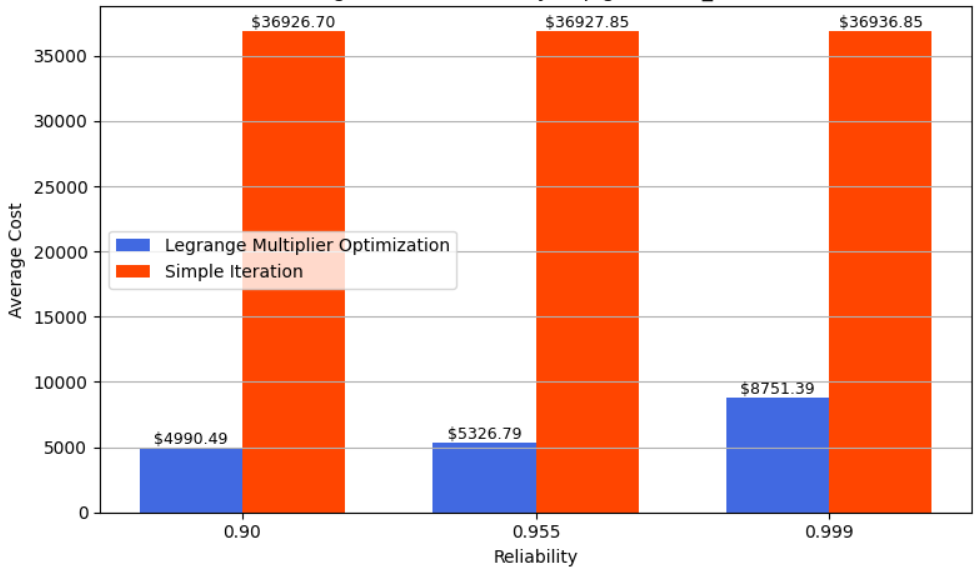
\includegraphics[width=0.8\textwidth]{figures/Epi_rel.png}
    \caption{Effect of varying reliability on total execution cost for the Epigenomics workflow using proposed algorithm and iterative approach}
    \label{fig:epigenomics-cost-rel}
\end{figure}

\begin{figure}[h!]
    \centering
    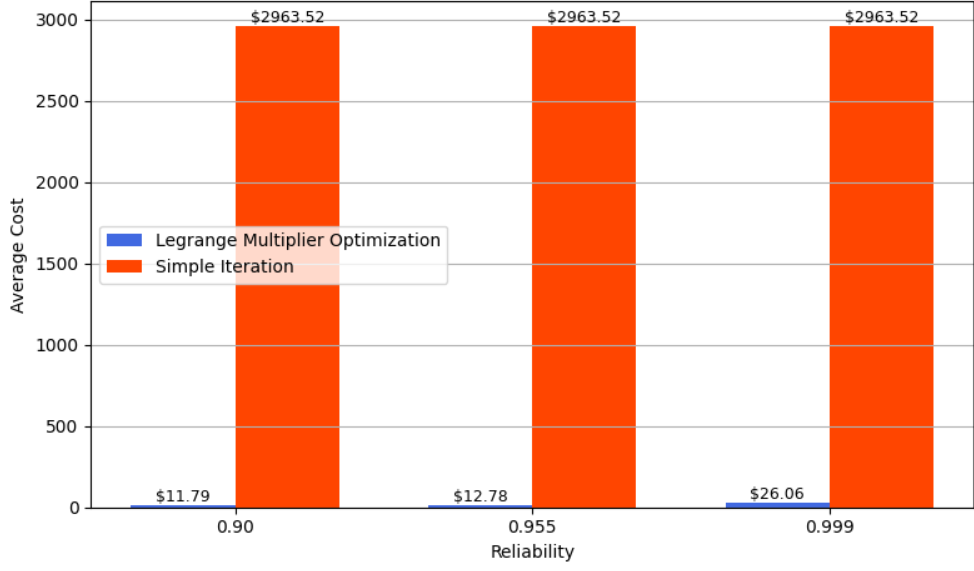
\includegraphics[width=0.8\textwidth]{figures/Siph_rel.png}
    \caption{Effect of varying reliability on total execution cost for the Sipht workflow using proposed algorithm and iterative approach}
    \label{fig:sipht-cost-rel}
\end{figure}

A two-way ANOVA was conducted to evaluate the effect of the chosen replication method and reliability level on the total execution cost. The results, summarized in Table~\ref{tab:anova}, show that the \textbf{method used for replica count estimation} has a statistically significant effect on cost (\textit{p} $< 0.001$). In contrast, the \textbf{reliability levels} and the \textbf{interaction between method and reliability} did not have a significant impact. This suggests that the choice of method—proposed algorithm vs. iterative—plays a much greater role in determining cost efficiency than the reliability constraint alone.

\begin{table}[h!]
    \centering
    \caption{Two-way ANOVA comparing cost across methods and reliability levels}
    \label{tab:anova}
    \begin{tabular}{lcccc}
        \toprule
        \textbf{Source} & \textbf{Sum of Squares} & \textbf{df} & \textbf{F-value} & \textbf{p-value} \\
        \midrule
        Method & $6.76 \times 10^{9}$ & 1 & 42.55 & $5.05 \times 10^{-10}$ \\
        Reliability & $1.82 \times 10^{7}$ & 2 & 0.057 & 0.944 \\
        Method $\times$ Reliability & $1.67 \times 10^{7}$ & 2 & 0.053 & 0.949 \\
      
        \bottomrule
    \end{tabular}
\end{table}




	
	
	\chapter{Conclusion}
	\label{sec_conclusion}
	
	This study presents an efficient and reliability-aware workflow scheduling framework that integrates replica count optimization and cost-effective task assignment under deadline constraints. By leveraging a combination of Lagrangian optimization for estimating optimal replica counts and a heuristic scheduler that considers VM eligibility, availability, and communication delays, the proposed method demonstrates substantial improvements in cost efficiency while meeting stringent reliability targets.

Experimental evaluations were conducted on three real-world scientific workflows—\textit{Montage}, \textit{Epigenomics}, and \textit{Sipht}—using VM configurations based on AWS EC2 instance data to ensure realism in modeling. Simulations performed under varying reliability levels (0.90, 0.95, 0.99) and increasing deadline flexibility showcased a clear trend: softer deadlines allow more relaxed task placement, reducing cost, while higher reliability thresholds predictably increase replication and cost. The results consistently showed that our optimization-based approach outperforms traditional iterative methods in terms of cost, especially under tight constraints.

Furthermore, statistical validation using two-way ANOVA confirmed that the choice of replica estimation method has a significant impact on cost, whereas variations in reliability level do not significantly affect it. This underscores the importance of a smart pre-allocation strategy in large-scale workflow environments.

Overall, the proposed approach enables scalable, reliable, and cost-aware execution of workflows in heterogeneous cloud environments. Future work can explore adaptive online scheduling, integration with spot pricing models, and energy-aware optimizations for further gains in sustainability and resource efficiency.

	
	\newcommand{\Extrachap}[1]{\chapter*{#1}\markboth{#1}{#1}%
		\addcontentsline{toc}{chapter}{#1}}
	
	\chapter*{References}
\addcontentsline{toc}{chapter}{References}
	
	\begin{enumerate}
    \item C. K. Swain and A. Sahu, "Reliability-ensured efficient scheduling with replication in cloud environment," \textit{IEEE Systems Journal}, 2022.

    \item E. Deelman, D. Gannon, M. Shields, and I. Taylor, “Workflows and e-Science: An overview of workflow system features and capabilities,” \textit{Future Generation Computer Systems}, vol. 25, no. 5, pp. 528–540, 2009.

    \item H. Topcuoglu, S. Hariri, and M.-Y. Wu, “Performance-effective and low-complexity task scheduling for heterogeneous computing,” \textit{IEEE Transactions on Parallel and Distributed Systems}, vol. 13, no. 3, pp. 260–274, 2002.
    
    \item J. Yu and R. Buyya, “Scheduling scientific workflow applications with deadline and budget constraints using genetic algorithms,” \textit{Scientific Programming}, vol. 14, no. 3–4, pp. 217–230, 2006.
    
     \item Q. Peng, H. Jiang, M. Chen, J. Liang, and Y. Xia, “Reliability-aware and deadline-constrained workflow scheduling in mobile edge computing,” in \textit{Proceedings of the 2022 IEEE International Conference on Communications (ICC)}, Chongqing, China, 2022.
     
    \item S. Bharathi, A. Chervenak, E. Deelman, G. Mehta, M. H. Su, K. Vahi, and N. Wilkins-Diehr, “Characterization of scientific workflows,” in \textit{2008 Third Workshop on Workflows in Support of Large-Scale Science}, 2008, pp. 1–10.

    \item S. Pandey, W. Voorsluys, S. Jha, and R. Buyya, “A particle swarm optimization-based heuristic for scheduling workflow applications in cloud computing environments,” in \textit{24th IEEE International Conference on Advanced Information Networking and Applications}, 2010, pp. 400–407.

   

\end{enumerate}
	
	
	\label{lastpage}
\end{document}